\documentclass[
	%parspace, % Térköz bekezdések közé / Add vertical space between paragraphs
	%noindent, % Bekezdésének első sora ne legyen behúzva / No indentation of first lines in each paragraph
	%nohyp, % Szavak sorvégi elválasztásának tiltása / No hyphenation of words
	%twoside, % Kétoldalas nyomtatás / Double sided format
	%draft, % Gyorsabb fordítás ábrák rajzolása nélkül / Quicker draft compilation without rendering images
	%final, % Teendők elrejtése / Set final to hide todos
]{elteikthesis}[2021/09/20]

% A minted csomag támogatott a forráskódok szedésére
% The minted package is also supported for source highlighting
%\usepackage[newfloat]{minted}

% Dolgozat metaadatai
% Document's metadata
\title{Kisvállalatokat segítő webáruház Angular keretrendszerben} % cím / title
\date{2021} % védés éve / year of defense

% Szerző metaadatai
% Author's metadata
\author{Magyar Dorina}
\degree{programtervező informatikus BSc}

% Témavezető(k) metaadatai
% Superivsor(s)' metadata
\supervisor{Fekete Anett} % belső témavezető neve / internal supervisor's name
\affiliation{PhD hallgató, MSc} % belső témavezető beosztása / internal supervisor's affiliation
%\extsupervisor{Külső Kornél} % külső témavezető neve / external supervisor's name
%\extaffiliation{informatikai igazgató} % külső témavezető beosztása / external supervisor's affiliation

% Egyetem metaadatai
% University's metadata
\university{Eötvös Loránd Tudományegyetem} % egyetem neve / university's name
\faculty{Informatikai Kar} % kar neve / faculty's name
\department{Programozási nyelvek és Fordítóprogramok\\ Tanszék} % tanszék neve / department's name
\city{Budapest} % város / city
\logo{elte_cimer_szines} % logo

% Irodalomjegyzék hozzáadása
% Add bibliography file
\addbibresource{thesis.bib}

% A dolgozat
% The document
\begin{document}

% Nyelv kiválasztása
% Set document language
\documentlang{magyar}
%\documentlang{english}

% Teendők listája (final dokumentumban nincs)
% List of todos (not in the final document)
%\listoftodos[\todolabel]

% Címlap (kötelező)
% Title page (mandatory)
\maketitle
\topicdeclaration

% Tartalomjegyzék (kötelező)
% Table of contents (mandatory)
\tableofcontents
\cleardoublepage

% Tartalom
% Main content
\chapter{Bevezetés} % Introduction
\label{ch:intro}

A \citeauthor{WebBeauty}(továbbiakban \citeauthor{WB}) lehetőséget kínál a kisvállalkozók által gyártott termékek bemutatására és árusítására. Mivel napjainkban menőt a kereslet a személyes webáruházak létrehozása iránt, ahol a saját termékeiket kívánják értékesíteni, ezt pedig a \citeauthor{WB} megfelelően kiszolgálja. Az webalkalmazás nem csak a felhasználók számára könnyen kezelhető, hanem egyben a tulajdonosnak is. Lehetőségük van arra, hogy egyszerűen menedzselhessék termékeiket és kapcsolatot tartsanak a lehetséges vásárlókkal. 

Számomra a témaválasztás célja egy személyesen ismert vállalkozó megkeresésén alapult, aki szívesen értékesítene az általam készített webáruházon keresztül a termékeit. Az alap problémát az vetette fel részemről, hogy egyénileg nem tudnám kiszolgálni az üzlettulajdonos által érkező folyamatos frissítési kéréseit. Ezt a felmerülő nehézséget úgy próbáltam megoldani, hogy a vállalkozó által is kényelmesen elérhetővé tegyem azokat a funkciókat, ami a webalkalmazás aktualizáltságát biztosítja. Továbbá a program képes a tulajdonos és a vásárló közötti közvetlen kapcsolat látszatát kialakítani a \citeauthor{chatbot}\footnote{egy szoftver alkalmazás, aminek a támogatásával közvetlen emberi kapcsolat helyett egy virtuális ’asszisztenssel’ kommunikáljon.} funkció segítségével. Mivel ez egy egyszerűbb webalkalmazás, ezért nem egy teljesen egyénileg gondolkozó mesterséges intelligencia(MI)\footnote{sokféle megközelítést találhatunk a definícióját illetően. Személy szerint azt gondolom, hogy az MI egy tudatos gondolkozásra alkalmas, emberi beavatkozás nélküli cselekvőképes létforma, amit a legtöbbször számítástechnikai eszközökhöz/gépekhez társítunk.} alapú chatbotról esik szó, hanem egy adatbázisban tárolt előre legenerált válaszokból álló szöveges adathalmazról beszélhetünk, ami kulcsszavas keresés segítségével zajlik.

\cleardoublepage

\chapter{Felhasználói dokumentáció} % User guide
\label{ch:user}

Az alkalmazás készítése során fontos szempont volt, hogy egy felhasználóbarát webáruházat hozzak létre. A webshop használata egyszerű letisztult felülettel rendelkező program olyan funkciókkal kiegészítve, amik megkönnyítik az átlagos vásárlók számára az oldal kezelését. A fejezet célja, hogy bemutassa az alkalmazás azon tulajdonságait, ami nem feltétlenül egyértelmű egy hétköznapi kliens számára. Ezzel is elősegítve a webalkalmazás gördülékeny felhasználását.


\section{Alkalmazás indítása} % Enumerations and lists

Egy hétköznapi felhasználó számára talán ez a legnagyobb kihívás a program használatával kapcsolatban. Az alkalmazás indítására két módszer közül választhatunk, amik a következőek:

\begin{compactenum}
	\item Megnyitni böngésző segítségével a weboldalt. 2.1.1. fejezet
	\item Megnyitni localhostról a projektet. 2.1.2 fejezet
\end{compactenum}

\bigskip
Mindkettő technikát részletes bemutatásra kerül a következő alfejezetekben.

\subsection{Alkalmazás indítás böngészőből}
Az első és legkönnyebben alkalmazható stratégia, hogy valamilyen előre telepített webböngésző (Chrome, Firefox, Opera..stb.) segítségével megnyitjuk az előre Amazon (AWS) szerverére telepített weboldalt. A felület ezen az url-címen érhető el: http://webbeauty.us-east-2.elasticbeanstalk.com

\subsection{Alklamazás indítása saját gépről}
Az előző  módszert azért neveztem könnyebben alkalmazhatónk, mert ha saját gépről szeretnénk indítani az alkalmazás nem csak le kell klónoznunk azt Github segítségével, hanem több különböző szoftvert kell telepítenünk mielőtt eltudnánk indítani magát a projektet. Magához a program fordításához szükségünk lesz a Node.js szoftverre, ami letölthető ingyenesen a nodejs.org eredeti honlapjáról. Továbbá még elengedhetetlen a gépünkről az Angular CLI. Ez egy parancssori interfész az Angular szoftverhez. Mivel a kód futtatásához szükségünk van rengetek eszközre, amely lefordítja és optimalizálja a kódot. A CLI ezt biztosítja a projekt számára. A kód fordításához szükségük lesz egy integrált fejlesztői környezetre. Én személy szerint a Visual Studio Code(rövidítve VS Code) nyílt forráskódú kódszerkesztőjét használtam az alkalmazás elkészítése során, így ezt fogom bemutatni.

A következő felsorolásban összefoglalom azokat a lépéseket, amik segítségével eljutunk a program saját gépről való indítását.

\begin{enumerate}
	\item\label{step:first} https://nodejs.org-ról töltsük le és telepítsük a számítógépre megfelelő .exe kiterjesztésű fájlt.
	\item https://github.com/magyardor/szakdolgozat2021 url-címen elérhető GitHub repository-t klónozzuk le az eszközünkre
	\item töltsük le, és telepítsük a Visual Studio Code nevezetű programot a https://code.visualstudio.com címről.
	\item nyissuk meg a VS code alkalmazást és installáljuk a következő bővítményeket: Angular Essentials, Material Icon Theme
	\item a VS code segítségével töltsük be a leklónozott projekt mappáját, és nyissuk meg egy új terminált
	\item a terminálba lépjünk be a szakdolgozat nevezetű mappájába és futtassuk le a következő parancssort: npm install -g @angular/cli
	\item ha ez sikeresen megtörtént akkor futtassuk le az npm i parancssort, aminek a segítségével letöltődnek azok a szükséges fájlok, amik nem szerepelnek az Angular CLI interfészben, de használatban vannak 
	\item mielőtt elindítanánk az alkalmazást be kell lépnünk a projekthez tartozó MongoDB adatbázisba és hozzá kell adnunk a hálózati hozzáférés nevezetű menüpont alatt a gépünk IP címét, különben nem tud csatlakozni a szerveroldalunk az alkalmazás által megjelenítendő adatokhoz
	\item a meglévő terminálunk mellé nyissunk meg egy újat és futtassuk le az egyikbe az npm run start a másikba az npm run start:server parancsokat, az előbbi a kliensoldalt, míg az utóbbi a szerveroldali kódokat futtatja és fordítja le
	\item ha sikeresen lefordult a kód, akkor a böngésző url helyére a localhost:4200 címet begépelve megkapjuk a webáruház oldalát
\end{enumerate}


\section{Alkalmazás kezelése} % Images and figures

Aliquam vehicula luctus mi a pretium. Nulla quam neque, maximus nec velit in, aliquam mollis tortor. Aliquam erat volutpat. Curabitur vitae laoreet turpis. Integer id diam ligula. Nulla sodales purus id mi consequat, eu venenatis odio pharetra. Cras a arcu quam. Suspendisse augue risus, pulvinar a turpis et, commodo aliquet turpis. Nulla aliquam scelerisque mi eget pharetra. Mauris sed posuere elit, ac lobortis metus. Proin lacinia sit amet diam sed auctor. Nam viverra orci id sapien sollicitudin, a aliquam lacus suscipit, Figure~\ref{fig:example-1}:

\begin{figure}[H]
	\centering
	\includegraphics[width=0.6\textwidth,height=100px]{elte_cimer_szines}
	\caption{Quisque ac tincidunt leo}
	\label{fig:example-1}
\end{figure}

\subsection{Webshop felület kezelése} % Framing figures

Ut aliquet nec neque eget fermentum. Cras volutpat tellus sed placerat elementum. Quisque neque dui, consectetur nec finibus eget, blandit id purus. Nam eget ipsum non nunc placerat interdum.

\begin{figure}[H]
	\centering
	\includegraphics[width=0.6\textwidth,height=100px,frame]{elte_cimer_szines}
	\caption{Quisque ac tincidunt leo}
\end{figure}

\subsection{Adminisztrációs felület kezelése} % Subfigures

In non ipsum fermentum urna feugiat rutrum a at odio. Pellentesque habitant morbi tristique senectus et netus et malesuada fames ac turpis egestas. Nulla tincidunt mattis nisl id suscipit. Sed bibendum ac felis sed volutpat. Nam pharetra nisi nec facilisis faucibus. Aenean tristique nec libero non commodo. Nulla egestas laoreet tempus. Nunc eu aliquet nulla, quis vehicula dui. Proin ac risus sodales, gravida nisi vitae, efficitur neque, Figure~\ref{fig:example-2}:

\begin{figure}[H]
	\centering
	\subcaptionbox{Vestibulum quis mattis urna}{
		\includegraphics[width=0.45\linewidth]{elte_cimer_szines}}
	\hspace{5pt}
	\subcaptionbox{Donec hendrerit quis dui sit amet venenatis}{
		\includegraphics[width=0.45\linewidth]{elte_cimer_szines}}
	\caption{Aenean porttitor mi volutpat massa gravida}
	\label{fig:example-2}
\end{figure}

Nam et nunc eget elit tincidunt sollicitudin. Quisque ligula ipsum, tempor vitae tortor ut, commodo rhoncus diam. Pellentesque habitant morbi tristique senectus et netus et malesuada fames ac turpis egestas. Phasellus vehicula quam dui, eu convallis metus porta ac.


\section{Rendelési folyamat} % Tables

Nam magna ex, euismod nec interdum sed, sagittis nec leo. Nam blandit massa bibendum mattis tristique. Phasellus tortor ligula, sodales a consectetur vitae, placerat vitae dolor. Aenean consequat in quam ac mollis. 

\begin{table}[H]
	\centering
	\begin{tabular}{ | m{0.25\textwidth} | m{0.65\textwidth} | }
		\hline
		\textbf{Phasellus tortor} & \textbf{Aenean consequat} \\
		\hline \hline
		\emph{Sed malesuada} & Aliquam aliquam velit in convallis ultrices. \\
		\hline
		\emph{Purus sagittis} &  Quisque lobortis eros vitae urna lacinia euismod. \\
		\hline
		\emph{Pellentesque} & Curabitur ac lacus pellentesque, eleifend sem ut, placerat enim. Ut auctor tempor odio ut dapibus. \\
		\hline
	\end{tabular}
	\caption{Maecenas tincidunt non justo quis accumsan}
	\label{tab:example-1}
\end{table}

\subsection{Vásárlással kapcsolatos információk} % Multi rows and multi columns

Mauris a dapibus lectus. Vestibulum commodo nibh ante, ut maximus magna eleifend vel. Integer vehicula elit non lacus lacinia, vitae porttitor dolor ultrices. Vivamus gravida faucibus efficitur. Ut non erat quis arcu vehicula lacinia. Nulla felis mauris, laoreet sed malesuada in, euismod et lacus. Aenean at finibus ipsum. Pellentesque dignissim elit sit amet lacus congue vulputate.

\begin{table}[htb]
	\centering
	\begin{tabular}{ | c | r | r | r | r | r | r | }
		\hline
		\multirow{2}{*}{\textbf{Quisque}} & \multicolumn{2}{ c | }{\textbf{Suspendisse}} & \multicolumn{2}{ c | }{\textbf{Aliquam}} & \multicolumn{2}{ c | }{\textbf{Vivamus}} \\
		\cline{2-7}
		& Proin & Nunc & Proin & Nunc & Proin & Nunc \\
		\hline \hline		
		Leo & 2,80 MB & 100\% & 232 KB & 8,09\% & 248 KB & 8,64\% \\
		\hline
		Vel & 9,60 MB & 100\% & 564 KB & 5,74\% & 292 KB & 2,97\% \\
		\hline
		Auge & 78,2 MB & 100\% & 52,3 MB & 66,88\% & 3,22 MB & 4,12\% \\
		\hline 
	\end{tabular}
	\caption[Rövid cím a táblázatjegyzékbe]{Vivamus ac arcu fringilla, fermentum neque sed, interdum erat. Mauris bibendum mauris vitae enim mollis, et eleifend turpis aliquet.}
	\label{tab:example-2}
\end{table}

\subsection{Rendelés leadása} % Long tables over multiple pages

Nunc porta placerat leo, sit amet porttitor dui porta molestie. Aliquam at fermentum mi. Maecenas vitae lorem at leo tincidunt volutpat at nec tortor. Vivamus semper lacus eu diam laoreet congue. Vivamus in ipsum risus. Nulla ullamcorper finibus mauris non aliquet. Vivamus elementum rhoncus ex ut porttitor.

\begin{center}
	\begin{longtable}{ | p{0.3\textwidth} | p{0.7\textwidth} | }
		
		\hline
		\multicolumn{2}{|c|}{\textbf{Praesent aliquam mauris enim}}
		\\ \hline
		
		\emph{Suspendisse potenti} & \emph{Lorem ipsum dolor sit amet}
		\\ \hline \hline
		\endfirsthead % első oldal fejléce
		
		\hline
		\emph{Suspendisse potenti} & \emph{Lorem ipsum dolor sit amet}
		\\ \hline \hline
		\endhead % többi oldal fejléce
		
		\hline
		\endfoot % többi oldal lábléce
		
		\endlastfoot % utolsó oldal lábléce
		
		\emph{Praesent}
		& Nulla ultrices et libero sit amet fringilla. Nunc scelerisque ante tempus sapien placerat convallis.
		\\ \hline
		
		\emph{Luctus}
		& Integer hendrerit erat massa, non hendrerit risus convallis at. Curabitur ultrices, justo in imperdiet condimentum, neque tortor luctus enim, luctus posuere massa erat vitae nibh.
		\\ \hline
		
		\emph{Egestas}
		& Duis fermentum feugiat augue in blandit. Mauris a tempor felis. Pellentesque ultricies tristique dignissim. Pellentesque aliquam semper tristique. Nam nec egestas dolor. Vestibulum id elit quis enim fringilla tempor eu a mauris. Aliquam vitae lacus tellus. Phasellus mauris lectus, aliquam id leo eget, auctor dapibus magna. Fusce lacinia felis ac elit luctus luctus.
		\\ \hline
		
		\emph{Dignissim}
		& Praesent aliquam mauris enim, vestibulum posuere massa facilisis in. Suspendisse potenti. Nam quam purus, rutrum eu augue ut, varius vehicula tellus. Fusce dui diam, aliquet sit amet eros at, sollicitudin facilisis quam. Phasellus tempor metus vel augue gravida pretium. Proin aliquam aliquam blandit. Nulla id tempus mi. Fusce in aliquam tortor.
		\\ \hline
		
		\emph{Pellentesque}
		& Donec felis nibh, imperdiet a arcu non, vehicula gravida nibh. Quisque interdum sapien eu massa commodo, ac elementum felis faucibus.
		\\ \hline
		
		\emph{Molestie}
		& Cras ullamcorper tellus et auctor ultricies. Maecenas tincidunt euismod lectus nec venenatis. Suspendisse potenti. Pellentesque pretium nunc ut euismod cursus. Nam venenatis condimentum quam. Curabitur suscipit efficitur aliquet. Interdum et malesuada fames ac ante ipsum primis in faucibus.
		\\ \hline
		
		\emph{Vivamus semper}
		& In purus purus, faucibus eu libero vulputate, tristique sodales nunc. Nulla ut gravida dolor. Fusce vel pellentesque mi, vel efficitur eros. Nunc vitae elit tellus. Sed vestibulum auctor consequat. 
		\\ \hline
		
		\emph{Condimentum}
		& Nulla scelerisque, leo et facilisis pretium, risus enim cursus turpis, eu suscipit ipsum ipsum in mauris. Praesent eget pulvinar ipsum, suscipit interdum nunc. Nam varius massa ut justo ullamcorper sollicitudin. Vivamus facilisis suscipit neque, eu fermentum risus. Ut at mi mauris.
		\\ \hline
		
		\caption{Praesent ullamcorper consequat tellus ut eleifend}
		\label{tab:example-3}		
	\end{longtable}
\end{center}
\cleardoublepage

\chapter{Fejlesztői dokumentáció}
\label{ch:impl}

\section{Webalkalmazás specifikáció}
\label{section:specification}
Az alkalmazás fő célja egy olyan működő webáruház bemutatása, ami MEAN (MongoDB, Express.js, Angular, és Node.js - solution stack)\cite{mean:stack} nevezetű szoftverköteg segítségével készült. A MEAN  megoldásverem ingyenes, nyílt forráskódú szoftverek halmaza, ami lehetőséget kínál dinamikus weboldalak készítésére. A webalkalmazás két fő részre osztható: kliensoldali és szerveroldali (idegen nyelven: front-end és back-end) részre. A kliensoldal leglényegesebb feladata, hogy a felhasználó által is látott weboldalt megjelenítse grafikai UI/UX (User Interface/User Experience) dizájn implementálásával. Nevezetesen egy olyan rendszer, ami képes a felhasználó számára felületet és élményt biztosítani. Miközben a szerveroldal elsődleges feladata az alkalmazás úgynevezett business logikájának a megvalósítása. Ezen felül képes az adatok feldolgozására és hitelesítésére is. A \ref{fig.picture-1}-es ábrán szeretném bemutatni, milyen módon épül fel a webalkalmazás, továbbá megismertetni a két oldal kommunikációs kapcsolatát.

\begin{figure}[H]
	\centering
	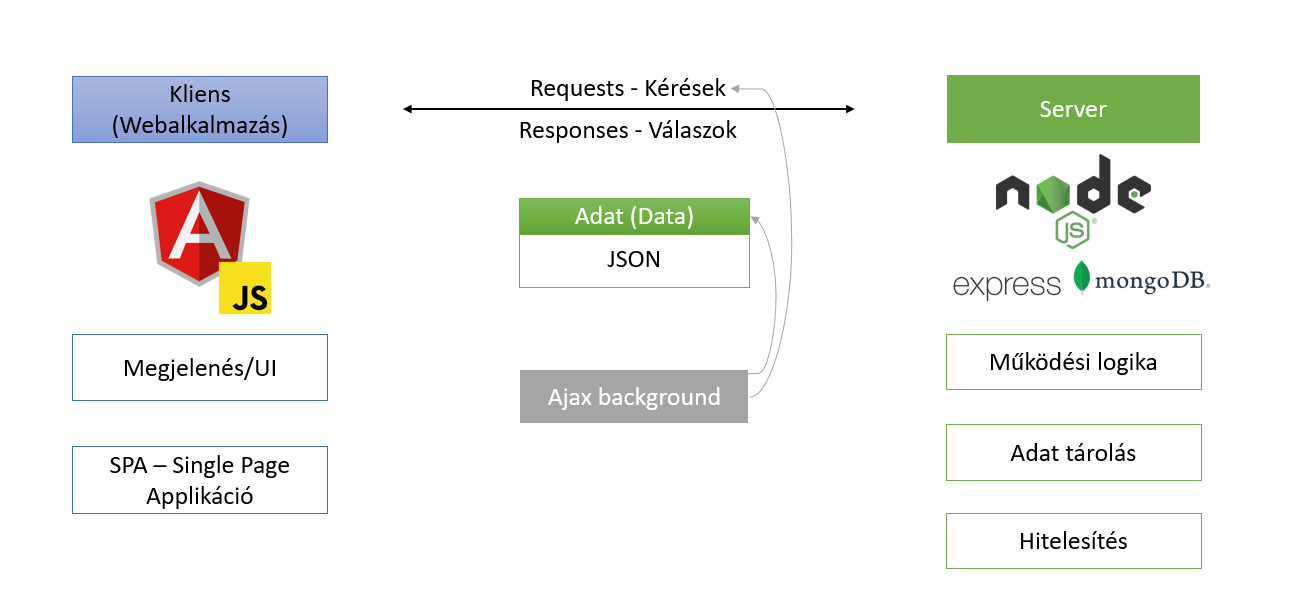
\includegraphics[width=1.0\textwidth]{images/alkalmazas_bemutatasa.png}
	\caption{Az alkalmazás rétegeinek bemutatása}
	\label{fig.picture-1}
\end{figure}

A \ref{fig.picture-1}-es ábrán látható, hogy a két oldal miképpen osztja meg az információkat egymás között. A front-end, pontosabban mondva a kliensoldal Angular\cite{angular:online} keretrendszerben, TypeScript\cite{ts} segítségével íródott. A front-end kommunikációja úgynevezett requestekkel, más néven kérésekkel (JSON formátumú adattovábbítással) a háttérben aszinkron módon történik, amire a szerveroldal response-okkal, vagyis válaszokkal felel. A back-end Node.js\cite{nodejs:online} szoftverrendszer alapú, ami Express.js\cite{express} keretrendszer segítségével íródott. Az adatok tárolásáért a MongoDB\cite{mongo} nevezetű adatbázis felel.

\bigskip
A következő blokkokban szeretném tételesen bemutatni a fentebb említett front-end és back-end oldalakon használt módszerek alkalmazását és működését. Ezen felül szándékomban áll ismertetni az általam alkalmazott szoftverek technikai tulajdonságait.

\section{Kliensoldalon használt technológiák bemutatása}
A klienoldal megjelenítéséhez az Angular keretrendszert használtam, aminek a segítségével dinamikus webalkalmazások hozhatóak létre. Az Angular egy nyílt forráskódú, Google által fejlesztett, JavaScript nyelven írt front-end keretrendszer. Ebben a fejezetben szeretném kellőképpen kifejteni, miért ezt a rendszert választottam az alkalmazás megírásához, ezen felül alaposabban bemutatni a működését és főbb tulajdonságait a \ref{fig.picture-2}-es ábra segítségével. 

\subsection{Angular keretrendszer}

\begin{figure}[H]
	\centering
	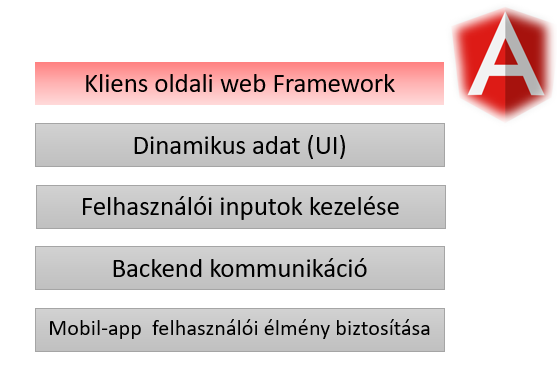
\includegraphics[width=1.0\textwidth]{images/angular_bemutatas.png}
	\caption{Az Angular keretrendszer bemutatása}
	\label{fig.picture-2}
\end{figure}

Az Angular egy kliensoldali keretrendszer, ennek köszönhetően képes feldolgozni és megjeleníteni a back-end felől érkező adatokat, aminek segítségével egy dinamikus webalkalmazást láthatunk a böngészőnkön keresztül. Ezt úgy tudja biztosítani, hogy képes kapcsolatot kialakítani a szerveroldallal. Továbbá lehetőséget nyújt a felhasználó által beérkezett adatok fogadására és kezelésére, ezen tulajdonga segítségével egy modern UI/UX felület készítésére alkalmazhatjuk. A program megírása során a 13.0.4 legújabb verziójú Angular CLI-t telepítettem. Mindezen jellemzői hozzátesznek ahhoz, hogy Single Page Application-nek (rövidítve: SPA)\cite{spa} nevezzük az általa támogatott weboldalakat. Olyan webhelyeket hívhatunk SPA-nak, amelyek egyetlen oldalra töltik be dinamikusan az adatokat, más szóval minden elemük egy oldalon található. Ennek köszönhetően a weboldalon való navigáláshoz nem kell betölteni külön DOM, vagyis Dokumentumobjektum-modelleket.

\section{Kliensoldal működése}
\label{section:client}
A weboldal felépítéséért és megjelenéséért a HTML, TypeScript és SCSS programozási nyelvek felelnek. A HTML feladata az alkalmazás tartalmi megjelenítése, az SCSS feladata pedig ezen tartalom formázása. A TypeScript biztosítja a felhasználó által kiadott utasítások végrehajtását. Az Angular keretrendszerben ez a három nyelv együttesen segít az oldalak megjelenítésében.

\subsection{Komponensek}
A komponensek\cite{components} a programkód logikai darabjai. Két fő eleme van:
\begin{compactenum}
	\item Sablon: az alkalmazás megjelenítéséért felel, ez tartalmazza a HTML-t
	\item Osztály: ebben szerepelnek a  metódusok és a tulajdonságok, ez a rész a TypeScript fájlokban van definiálva
\end{compactenum}

\subsection{Modulok}
Az Angular alkalmazás moduláris és saját moduláris rendszerrel rendelkezik, amit NgModulesnak\cite{ngmodules} nevezünk. Ennek a modulnak a metaadatai segítségével különböző komponenseket, direktívákat és szolgáltatási(angolul: service) fájlokat csoportosíthatunk. Az NgModule-nak öt ilyen metaadata van, aminek a használatával kategorizálhatjuk a komponenseinket felhasználás szerint.

Az NgModule metaadatai:

\begin{itemize}
	\item deklarációk (declarations): az itt szereplő komponensek kifejezetten ahhoz a modulhoz tartoznak, ahol létrehoztuk őket.
	\item exportok (exports): a deklarációban használt komponensek azon részhalmaza, amiknek láthatónak kell lennie máshol létrehozott komponensek számára.
	\item importok (imports): olyan modulokat tartalmaz, amiket a deklarációnál implementált komponensek használnak.
	\item szolgáltatók (providers): olyan osztályok szerepelnek itt, amelyek létrehozzák és menedzselik a service objektumokat első alkalomkor, amikor az Angularnak szüksége van a függőségek feloldásához.
\end{itemize}

\subsection{Interfészek}
Az interfészek\cite{interface} olyan specifikációk az Angular keretrendszerben, amelyek egy osztály által megvalósítandó tulajdonságok és metódusok összefüggő halmazát határozzák meg. Tehát a segítségével létrehozható pár alapvető szabály a tulajdonságokra és a metódusokra, amiket használunk az osztályon belül.

\subsection{Service files}
A projektben a service files\cite{service} tartalmazza azokat a függvényeket, amiknek a segítségével kapcsolatot alakíthatunk ki a szerveroldallal. Ezek a fájlok tartalmaznak bizonyos kéréseket, amiknek a segítségével a felhasználó elindíthatja az adatlekérés folyamatát. A függvények kigyűjtésének célja, hogy egyszerűbben elérhetőek legyenek több komponens számára, ezzel lehetőséget biztosít a többszöri felhasználásra. Továbbá egyszerűsíti a metódusok megváltoztatását más keretrendszer használata esetén.

\subsection{Admin mappa}
Ez a mappa tartalmazza az adminisztrációs oldal megjelenítéséhez szükséges fájlokat, elkülönítve a többi komponenstől. Erre azért volt szükség, mert a két oldal szerkezeti felépítése eltérő egymástól, továbbá segítette a fejlesztés során ezeket elszeparálva tartani.

\subsection{Pages mappa}
A webalkalmazás olyan komponensei találhatóak ebben a mappában, amik nincsenek bejelentkezés funkció mögé rejtve. Tehát az elérésükhöz nem szükséges autentikáció. Az áruház öt fő oldala található meg itt.

\begin{compactitem}
	\item Főoldal/Kezdőlap: összefoglalja a hírek és a termékek oldalát.
	\item Hírek: az oldal üzemeltetője által megosztott fontosabb információk.
	\item Termékek: minden olyan termék, amit eladásra szánnak.
	\item Rólunk: az oldal üzemeltetőjével kapcsolatos információk, elérhetőségek.
	\item Bevásárlókosár: a felhasználó által kiválasztott termékek.
\end{compactitem}

\subsection{Oldalak közötti navigáció}
Az oldalak közötti koordinálást\cite{navigation} az előbbiekben kifejtett modulok egyike kezeli. Angularban a legjobb mód az, hogy ha a routerbe betöltést és konfigurálást különállóan kezeljük. A router egy szolgáltatás, ami biztosítja az oldalak közötti navigációt. A konfigurálás az AppRoutingModule-ban zajlik, míg a betöltés a legfelső szintű modulban azaz az AppModule-ban van importálva, ami útválasztóként is szolgál.

\subsection{Shared mappa}
A Shared mappa tartalmazza azokat a komponenseket és Angular kiegészítő csomagokat, amik több oldalon is megjelenítésre kerülnek. Ezek a komponensek és package-ek a következők:

\begin{itemize}
	\item Angular Material\cite{material}: egy felhasználói felület (UI) komponens könyvtár. Az Angular Material használata gyorsítja a fejlesztési folyamatot és egy konzisztens, elegáns felületet biztosít.
	\item Alert üzenetek: segítségével a felhasználó által elindított folyamatok állapotáról nyújthatunk információt.
	\item Nyelvválasztás: lehetőséget biztosít az oldalon található adatok többnyelvű megjelenítésére.
	\item Vissza gomb és az Ugrás a tetejése gomb: a nevükből kiindulva olyan gombok amik lehetőséget biztosítanak az oldalak navigálásra a felhasználók számára.
	\item Chatbot: animációval rendelkező beszélgetési felület, ami lehetőséget nyújt arra, hogy a felhasználó gyors információt szerezzen az adott szolgáltatásokkal kapcsolatban. A chatbot részletes bemutatása a (\ref{section:sourcecode})-es fejezet Kliensoldali forráskódok (\ref{subsection:clientsource}) alfejezetében található.
\end{itemize}

\subsection{Egyéb fájlok és mappák}
Ebben a blokkban szerepel minden olyan fájl, ami kiegészítő funkcióként szolgál a többi fájl számára.

\begin{itemize}
	\item Assets mappa: minden olyan képfájlt tartalmaz, amit nem dinamikusan kapunk a szervertől. Ilyen képek például az oldalon használt logók és borítóképek.
	\item Enviroments mappa: az ebben szereplő fájlok tartalmazzák a szerveroldal eléréséhez szükséges URL címet.
	\item Theme mappa: olyan stílusfájl, ami a komponensekben használt színek gyűjteményét tartalmazza.
	\item \verb|style.scss|: minden olyan stíluselem leírása, amit a komponensek közösen használnak.
\end{itemize}

\section{Szerveroldalon használt technológiák bemutatása}
A szerveroldalon használt (a \ref{section:specification}-es alfejezetben már említett) módszerek kiválasztása előtt kulcsfontosságú szempontnak tartottam, hogy az Angular keretrendszerhez megfelelő kompatibilitással rendelkezzenek, és alkalmazni tudjam őket a szakdolgozat elkészítése során. A következő technológiák mind olyan szoftverek, keretrendszerek vagy adatbázisszerverek, amikhez számtalan  dokumentáció elérhető az interneten, ezzel támogatva a későbbiekben létrehozott projekteket. A következő felsorolásban összefoglalásképpen összegyűjtöttem az alkalmazásban fellelhető, általam használt szoftvereket és verziószámukat:

\begin{compactitem}
	\item Node.js: 14.15.4
	\item Express.js: 4.17.1
	\item Mongoose: 6.0.12
	\item MongoDB Atlas
\end{compactitem}

\bigskip
A fejezet további részében szeretném ismertetni a fentebb felsorolt technológiák jellegzetes tulajdonságait, főbb jellemzőit további ábrák segítségével.

\subsection{Node.js szoftverrendszer}

\begin{figure}[H]
	\centering
	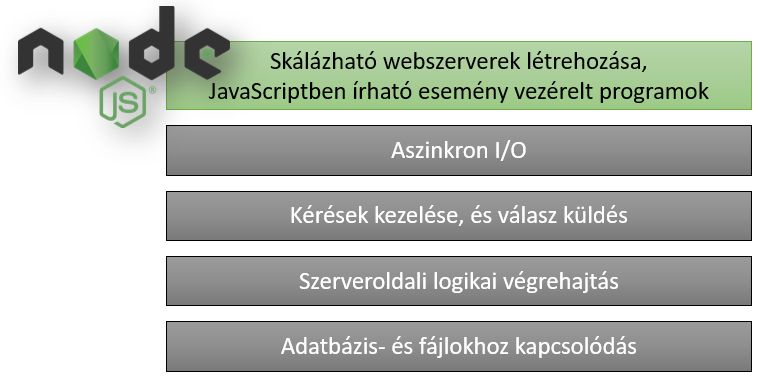
\includegraphics[width=1.0\textwidth]{images/nodejs_bemutatasa.png}
	\caption{Node.js bemutatása}
	\label{fig.picture-3}
\end{figure}

A webáruház back-endjének megírásánál 14.15.4-es verziójú Node.js szoftverrendszert használtam. A \ref{fig.picture-3}-as ábrán látható a Node.js bemutatása, ami összefoglalja a szoftverrendszer fontosabb jellemzőit. Az illusztráció első dobozában olvasható, hogy a Node.js skálázható webszerverek létrehozására alkalmas, más szóval egy olyan rendszert tudunk létrehozni a támogatásával, ami több felhasználót képes egyidejűleg kiszolgálni. Ezenfelül JavaScript nyelv segítségével olyan programok írhatóak, amelyek a komponensek közötti eseményinterakciókat tekintik alapul, más szóval eseményvezérelt programok megírására alkalmasak (ilyen például egy egérkattintás vagy billentyűleütés). Folytatólag a Node.js aszinkron tulajdonságával lehetővé teszi, hogy a kliensoldalról érkező kérések várakozási sorrendbe kerüljenek, ennek következtében a kliensoldal tovább folytathatja a feladatát. 

\subsection{Express.js keretrendszer és Mongoose programozási könyvtár}

\begin{figure}[H]
	\centering
	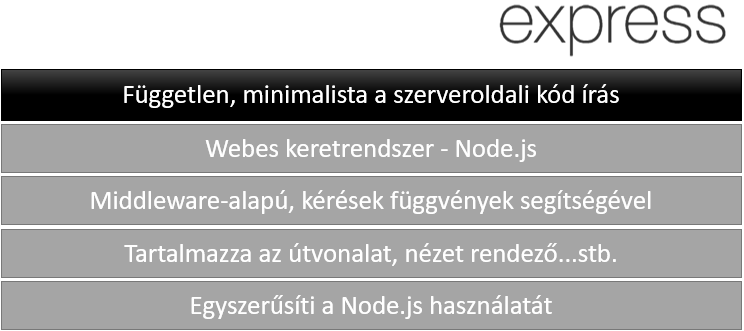
\includegraphics[width=0.8\textwidth]{images/express_bemutatasa.png}
	\caption{Express bemutatása}
	\label{fig.picture-4}
\end{figure}

A szerveroldal áttekinthetőbb és olvashatóbb kódírása érdekében a webáruház fejlesztése során az Express.js 4.17.1-es verzióját használtam. Az Express egy webes keretrendszer, amely a Node.js nehézség nélküli használatára lett fejlesztve. A \ref{fig.picture-4}-es ábrán látható az Express attribútumainak ismertetése. Az Express egy Middleware-típusú rendszer, következésképpen lehetővé teszi a MongoDB adatbázisszoftverhez való zavartalan kapcsolódást a Mongoose\cite{mongoose} 6.0.12 verziójával kiegészítve, ami egy JavaScript-ben írt objektumorientált programozási könyvtár.

\subsection{MongoDB adatbázisszerver}

\begin{figure}[H]
	\centering
	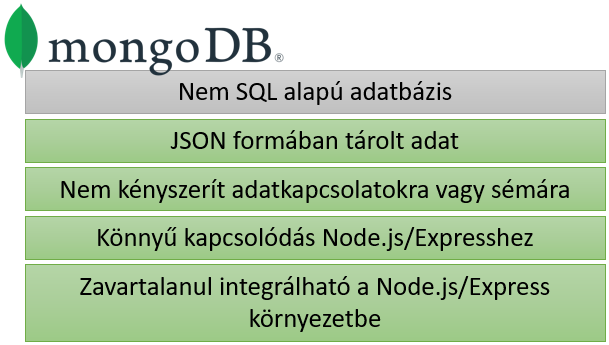
\includegraphics[width=0.8\textwidth]{images/mongodb_bemutatasa.png}
	\caption{MongoDB bemutatása}
	\label{fig.picture-5}
\end{figure}

A MongoDB egy nyílt forráskódú, NoSQL\cite{nosql} adatbázisszerverek közé sorolt szoftver a \ref{fig.picture-5}-ös ábrán látottak szerint. A nevéből következtetve ez nem egy SQL típusú adatbázisrendszer. Jellemzően nem rekordokat és táblázatokat tárolnak, mint az SQL típusú szerverek, hanem független dokumentumokat és gyűjteményeket archiválnak. A NoSQL típusú adatbázisok többségében JSON\cite{json} formátumú adatok tárolására alkalmasak. A JSON(JavaScript Object Notation) nyelvfüggetlen kapcsolatot biztosító, szöveges alapú szabványt alkalmazó programozási nyelv. Következésképpen a request és response folyamatok egyszerűsített és gyors működését képes biztosítani, mindeközben lehetővé teszi a kliensoldalon megjelenítendő információk könnyebb feldolgozását. 
\bigskip

\subsection{NoSQL és SQL adatbázisok összehasonlítása}

A \ref{fig.picture-6}-os ábrán szándékozom röviden bemutatni és összehasonlítani a nem SQL és az SQL alapú adatbázisokat jellegzetes tulajdonságaik szerint.

\begin{figure}[H]
	\centering
	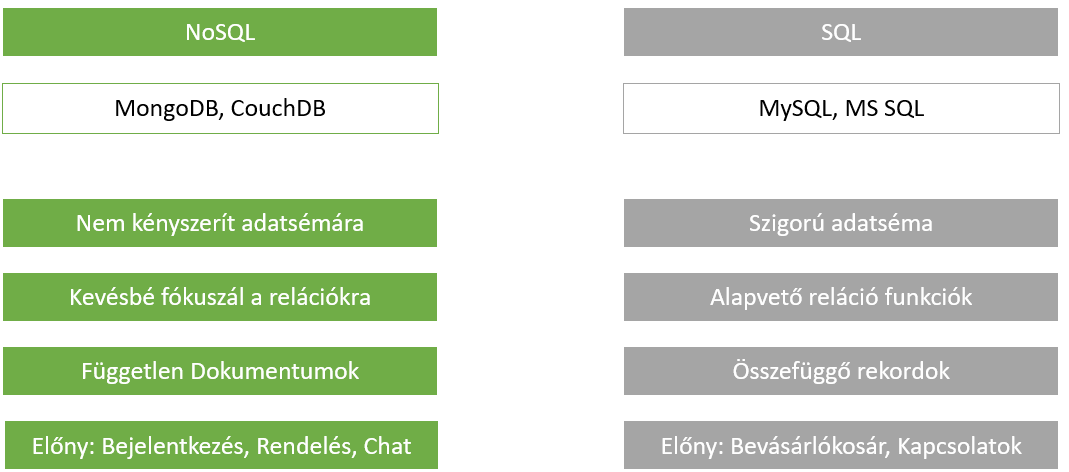
\includegraphics[width=1.0\textwidth]{images/nosql_bemutatasa.png}
	\caption{NoSQL és SQL adatbázisok összehasonlítása}
	\label{fig.picture-6}
\end{figure}

A \ref{fig.picture-6}-os ábrán megfigyelhető szempontok szerint egy webáruházban kezelt adatok tárolására a NoSQL adatbázisok kifejezetten alkalmasak. A NoSQL adatbázisszerverek jellemző tulajdonságai kulcsfontosságú szempontokkal szolgáltak a webáruház adatbázisának kiválasztásánál.

\subsection{Alkalmazás adatbázisának bemutatása}
Az alábbi \ref{fig.picture-7}-es ábrán látható az alkalmazásban használt adatbázis tervezete. Az illusztrációt osztály diagramként készítettem el. A NoSQL adatbázis típusnak köszönhetően az osztályoknak nem feltétlen kell kapcsolatot kialakítaniuk egymás között. Az adatbázisban hat darab gyűjtemény található. A hat gyűjtemény közül csak kettő áll kapcsolatban egymással, mégpedig a termékek listája és a termékek csoportja. A kapcsolat egy a sokhoz típusú, mivel egy csoporthoz több termék kapcsolódhat, de egy termékhez csak egy csoport.
\begin{figure}[H]
	\centering
	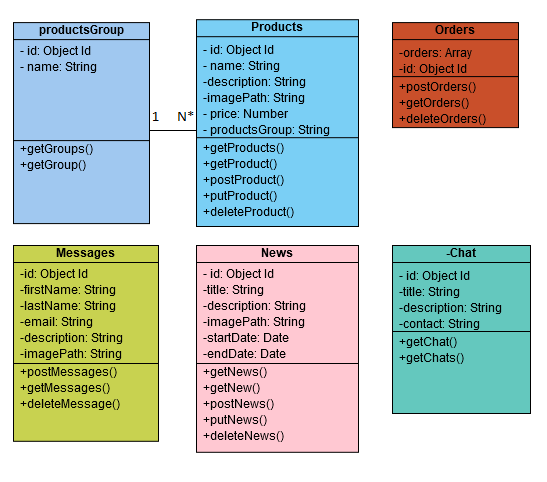
\includegraphics[width=1.0\textwidth]{images/class_diagram.PNG}
	\caption{Adatbázis - class diagram}
	\label{fig.picture-7}
\end{figure}

\section{Szerveroldal működése}

Ebben a fejezetben részletesen prezentálom az alkalmazás szerveroldali működését, például milyen request hívások találhatóak a kódban, hogyan létesít kapcsolatot a webalkalmazás az adatbázissal, stb., valamint külön kitérek az adminisztrációs oldalon található autentikációra is.

\subsection{REST API - Végpont tervek bemutatása}
\label{subsection:restapi}

A webáruház megírása során REST API-t (Representational State Transfer Application Programming Interface)\cite{restapi}, architekturális módszert használtam. A REST API-k komponensek összekapcsolására alkalmazzák, könnyű és rugalmas szolgáltatást biztosítva. Az API olyan szabályrendszert jelent, ami meghatározza az alkalmazások számára ilyen módon kapcsolódjanak és kommunikáljanak egymással. Lehetővé teszi a kliensoldalon található szolgáltatások számára, hogy hozzáférjen a szerveroldali erőforrásokhoz. Az alkalmazás tervezési fázisában ennek a két oldalnak függetlennek kell lennie egymástól. A kliensoldal számára egyetlen információnak a szerveroldal eléréséhez szükséges URL címének kell elérhetőnek lennie. Ugyan úgy, ahogy a szerveroldalnak sem szabad módosításokat végeznie a kliensoldalon, azon kívül, hogy az adatokat HTTP-n keresztül továbbítják egymásnak. Az adatok továbbítására az Angular által biztosított HttpClient\cite{http} szolgáltatási osztályt használja az alkalmazás. Ennek az osztálynak a segítségével fogja el a kimenő kérések és bejövő válaszokat az alkalmazás számára. A kliensoldal számos kérést képes elindítani, ezek közül az alkalmazásban használt kérések a következők:

\begin{compactitem}
	\item GET: lekérdezi az adatbázisban szereplő listákat
	\item POST: megkéri az adatbázist, hogy adja hozzá a listához az elküldött adatokat
	\item PUT: megkéri az adatbázist, hogy módosítsa a listában szereplő adatot az elküldött adatokra
	\item DELETE: megkéri az adatbázist, hogy az elküldött tulajdonságúval rendelkező adat kerüljön törlésre
\end{compactitem}

\bigskip
Az alábbi illusztráción szeretném bemutatni az alkalmazásban használt REST API hívásokat, ennek okán a \ref{fig.picture-8}-as ábrán láthatók a programban megírt végpontok.

\begin{figure}[H]
	\centering
	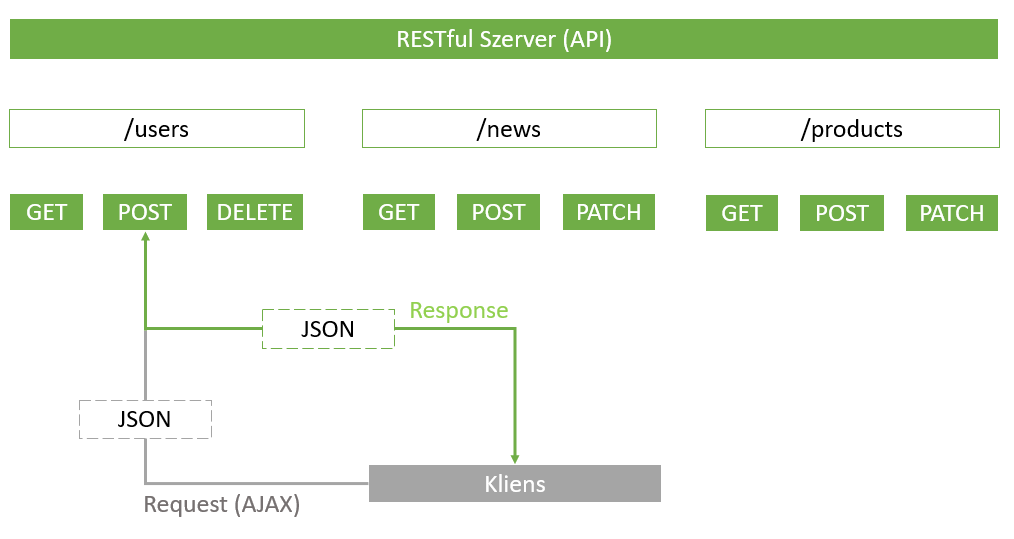
\includegraphics[width=1.0\textwidth]{images/restapi_bemutatasa.png}
	\caption{Adatkezelés}
	\label{fig.picture-8}
\end{figure}

A grafikán megfigyelhető hét különböző végpont, amelyek az autentikáció, hírek, termékek, termékcsoportok, üzenetek, chatek és rendelések funkciókhoz kapcsolódnak. Az illusztrációt figyelemmel kísérve látható, hogy nem minden végpont rendelkezik ugyanazokkal a kérésekkel. Szemléltetésképp vegyük figyelembe a hírekhez vonatkozó kéréseket, amik a GET, POST, PATCH és DELETE függvények, ezzel szemben a autentikációhoz kizárólag POST kérés tartozik. Ennek kifejezetten egy oka van, mégpedig az, hogy a webáruház egyes adatait nem szükséges módosítani tudni kliensoldalról.

\bigskip
A REST API-t megismerve és ezt az információt felhasználva a \ref{fig.picture-9}-es ábrán látható, miképpen éri el a felhasználó által kezdeményezett kérés az adatbázist és hogyan kap választ.

\begin{figure}[H]
	\centering
	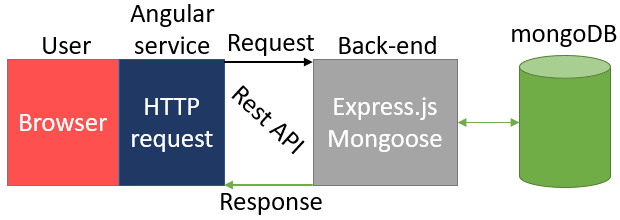
\includegraphics[width=1.0\textwidth]{images/kapcsolat_szerver_bemutatas.png}
	\caption{Kapcsolat a szerverrel}
	\label{fig.picture-9}
\end{figure}

A \ref{fig.picture-9}-es ábrával és az alább található alkalmazásban szereplő kódsorok segítségével szeretném bemutatni, hogy a felhasználó által indított kérés milyen sorrendben jut el az adatbázishoz és miképpen tér vissza a felhasználóhoz.

\bigskip
A felhasználó interakcióba lép a felülettel. Ilyen interakció lehet például a~\ref{src:html}-es forráskódban szereplő gomb megnyomása. A gombra kattintás következményeként meghívásra kerül a hozzá tartozó TypeScript programozási nyelv segítségével megírt a \ref{src:ts}-es forráskódban szerepelő függvény. Ez a függvény meghívja egy szolgáltatási fájl metódusát és adatokat ad át a számára.

\lstset{caption={Felhasználói interakció - HTML fájl}, label=src:html}
\begin{lstlisting}[language=html]
	<form style="margin-top: 2rem;" [formGroup]="form" (submit)="onAddMessage()" *ngIf="!isLoading">
	....
	<button class="btn-secondary" type="submit" [disabled]="!confirmed.checked">
	{{'GENERIC.ACTION.SEND' | translate}}
	</button>
\end{lstlisting}

\lstset{caption={Függvényhívás - TypeScript fájl}, label=src:ts}
\begin{lstlisting}[language=JavaScript]
	onAddMessage(): void {
		if(this.form.invalid) {
			this.alertService.warn('ALERT.WARN.INVALID_FORM');
			this.form.markAllAsTouched();
			this.isLoading = false;
			return;
		}
		this.isLoading = true;
		this.contactService.sendMessage(
		this.form.value.firstName,
		this.form.value.lastName,
		this.form.value.email,
		this.form.value.description,
		this.form.value.image,
		)
		this.isLoading = false
		this.form.reset();
	}
\end{lstlisting}

Az előbb említett \ref{src:ts}-es forráskódban szereplő függvény átadja az adatokat a kliensoldalon található Service fájl \verb|sendMessage()| nevezetű függvényének. Ez a fájl tartalmazza a \ref{src:service}-as forráskódban szereplő kódsort.

\lstset{caption={HttpClient POST request - Service TypeScript fájl}, label=src:service}
\begin{lstlisting}[language=JavaScript]
	sendMessage(
	firstName: string, 
	lastName: string, 
	email: string, 
	description: string, 
	image: File | string
	){
		const messagesData = new FormData();
		messagesData.append("firstName", firstName);
		messagesData.append("lastName", lastName);
		messagesData.append("email", email);
		messagesData.append("description", description);
		messagesData.append("image", image, firstName);
		this.http.post<{message: string, messages: Messages}>
		(environment.apiUrl + "messages", messagesData)
		.subscribe(responseData => {
			const messages: Messages = {
				id: responseData.messages.id,
				firstName: firstName,
				lastName: lastName,
				email: email,
				description: description,
				imagePath: responseData.messages.imagePath,
			};
			this.messages.push(messages);
			this.msgUpdate.next([...this.messages]);
			this.alert.success('ALERT.SUCCESS.ADD');
			this.router.navigate(["/contact"]);
		}, error => {
			this.alert.error(error.error.message);
		});
	}
\end{lstlisting}

Ebben a kódrészletben látható, ahogyan a kliens oldal HttpClient szolgáltatási osztály POST kérés segítségével a megadott útvonalon küld egy REST API hívást a szerveroldal felé.

\bigskip
A szerveroldal fogadja ezt a kérést és továbbítja a MongoDB felé. A \ref{src:express}-es forráskódban Express - JavaScript nyelv segítségével megírt kódrészletben ez szerepel.

\lstset{caption={Express POST végpont - JavaScript}, label=src:express}
\begin{lstlisting}[language=JavaScript]
	exports.postMessages = (req, res, next) => {
		const url = req.protocol + "://" + req.get("host");
		const msg = new Messages({
			firstName: req.body.firstName,
			lastName: req.body.lastName,
			email: req.body.email,
			description: req.body.description,
			imagePath: url + "/images/messages/" + req.file.filename,
		});
		msg.save().then(result => {
			res.status(201).json({
				message: "Message added successfully",
				messages: {
					...result,
					id: result._id
				}
			});
		});
	}
\end{lstlisting}

Kliensoldalon és szerveroldalon egyaránt látható a felhasználó által elindított kérés státuszát tartalmazó információ. A front-enden egy úgynevezett AlertService komponens segítségével kap visszaigazolást az elindított kérés befejezéséről. A back-end oldalon a \verb|res.status(201)| kódrészlet segítségével kapunk visszaigazolást a kérés befejezésével kapcsolatban.

\bigskip
A webalkalmazásban szereplő további REST API hívásokat tartalmazó példakódsorok a \ref{section:sourcecode}-es fejezet Szerveroldali forráskódok (\ref{subsection:serversource}) nevezetű alfejezetében találhatóak.

\subsection{Hitelesítés - Az adminisztrációs felület védelme}
Az alkalmazás megírása során szándékosan egy olyan webáruház létrehozása volt a célom, ami időszerű adatok kezelését tudja biztosítani. Következésképpen egy olyan felület megvalósítása, amely nem igényel az oldal üzemeltetéséhez programozói segítséget. Ennek okán a program tartalmaz egy adminisztrációs oldalt, amely biztosítja a webalkalmazásban dinamikusan megjelenő adatok aktualitását, továbbá a leadott rendelések és vásárlók által elküldött üzenetek megjelenítésére is szolgál. Kifejezetten ennek a blokknak védelmére került bele külön hitelesítési\cite{hitelesites} felület.

\bigskip
A \ref{fig.picture-10}-es grafikán található az engedélyezési folyamat elméleti működése.

\begin{figure}[H]
	\centering
	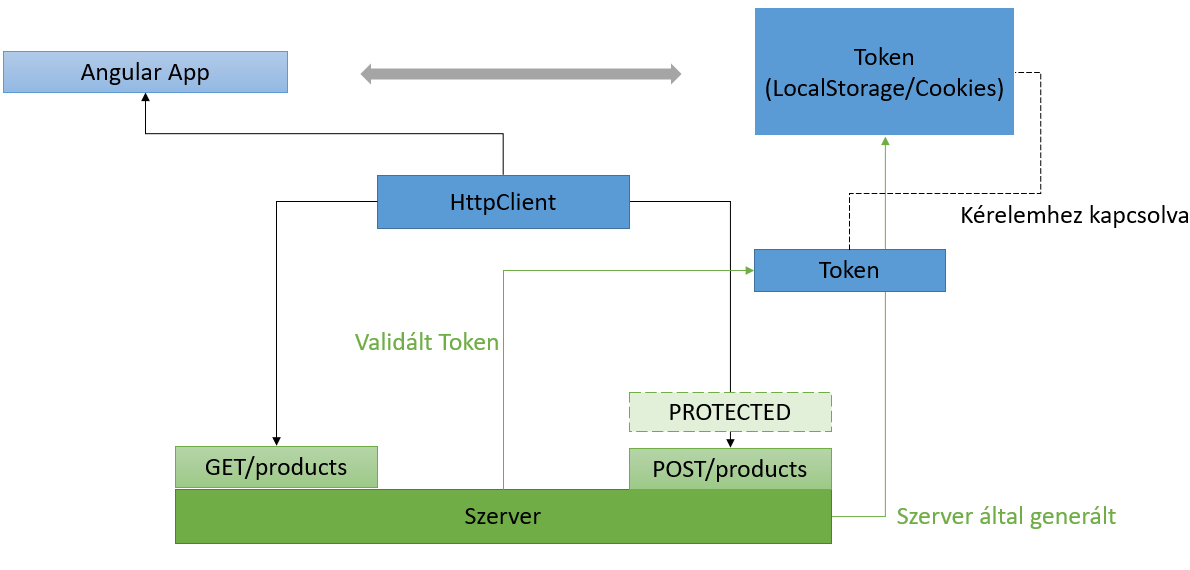
\includegraphics[width=1.0\textwidth]{images/hitelesites_bemutatasa.png}
	\caption{Hitelesítés}
	\label{fig.picture-10}
\end{figure}

Az illusztráción ábrázolt hitelesítési folyamat a következőképpen történik. Az alkalmazás front-endről érkező GET/products kérésre engedélyezés nélkül kap választ a szervertől, mivel a webáruházban bejelentkezés hiányában is hozzáférhetővé kell tenni a termékek listáját. Ezzel szemben a POST/products kérés nem következhet be hitelesítés nélkül. Tehát bejelentkezés során a szerver generál egy úgynevezett tokent és elmenti a LocalStorage-ba, amit az új termék hozzáadása kérésnél ellenőriz. Az alkalmazásban ez a hitelesítési funkció a következőképpen valósul meg:

Ennek a funkciónak a létrehozásánál két kiegészítő package-et, \textit{bcryptjs}-t és \textit{jsonwebtoken}-t használ a programkód. Az előbbi lehetőséget nyújt bizonyos adatok titkosítására (ilyen adat például a belépéshez szükséges jelszó), az utóbbi pedig bizonyos REST API kérések érvényesítésére alkalmas. Mikor létrehozásra kerül egy új felhasználó, a bcrypt package egy úgynevezett hasító metódusát hívja meg a program, aminek segítségével az új felhasználó jelszava titkosítva kerül be az adatbázisba. Ennek az az oka, hogy idegenek számára olvashatatlanná váljon ez az információ. Viszont ezzel probléma adódik a későbbiekben. Mivel, ha titkosítva kerül be az adatbázisba, az oldalra történő belépéskor nem elegendő összehasonlítani a begépelt adatott az adatbázisban tárolt adattal. Erre a problémára szolgál megoldásképp a bcryptjs \verb|compare| metódusának használata. Ennek a metódusnak segítségével összehasonlításra kerül az adott felhasználó adatbázisban szereplő titkosított jelszava és a begépelt jelszó hasított változata. Ennek köszönhetően, ha pont a megfelelő karaktereket gépeljük be, akkor a begépelt adat titkosított változatának megegyezőnek kell lennie az adatbázisban található adattal.

Mindent összevetve az adminisztrációs felület védve van az illetéktelen felhasználók belépésétől és bizonyos funkciók végrehajtásától.

\section{Az alkalmazás megjelenése}
Az oldal megjelenéséhez kapcsolatos színvilág, és vizuális elemek nagy részben a saját munkáim. Az összes látványelem, mint például a logó vagy az oldalon található képek, az Adobe Photoshop\cite{photoshop} 2019-es programjával készültek. Az alkalmazásban szereplő ikonok a Google Icons - Material icons\cite{material} segítségével kerültek megjelenítésre.

\subsection{Figma szoftver - oldalvázlatok}
Az alkalmazás fejlesztése előtt a megjelenő oldalakra tervezett drótvázterveket a Figma\cite{figma} nevezetű vektorgrafikus szerkesztő segítségével készítettem. A tervezés során meghatároztam, és összegyűjtöttem az alkalmazás színvilágát, ami a \ref{fig.picture-11}-es ábra bal oldalán látható. Ezek a színek globálisan kerültek implementálásra a kódon belül. Ez azt jelenti, hogy ha egyes színek lecserélésre kerülnek, akkor az alkalmazáson belül az adott színek az újonnan megadott színekként jelennek meg. Ezen felül olyan elemek kerültek megtervezésre, mint például az értesítő üzenetek vagy a \ref{fig.picture-11}-es ábra jobb oldalán látható gombok.
\begin{figure}[H]
	\centering
	\subcaptionbox{Globális színek}{
		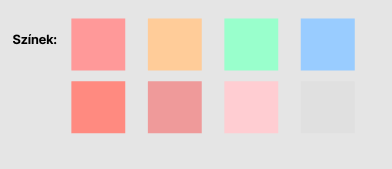
\includegraphics[width=0.45\textwidth]{images/szinek.png}}
	\hspace{5pt}
	\subcaptionbox{Gombok megjelenése}{
		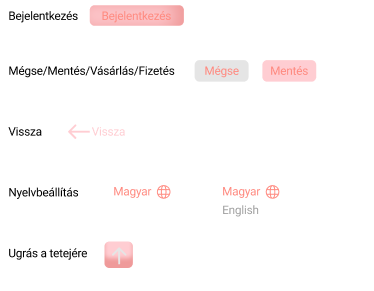
\includegraphics[width=0.45\textwidth]{images/gombok.png}}
	\caption{Figma kiegészítő elemek tervezete}
	\label{fig.picture-11}
\end{figure}

Az alkalmazásban megjelenő oldalak vázlatát is elkészítettem, ami a \ref{fig.picture-12}-es ábrán látható. Ha az ábrán szereplő két képet összehasonlítjuk az alkalmazásban megjelenő oldalakkal, akkor észrevehető mekkora különbség van az oldalvázlatok és az alkalmazásban szereplő végleges megjelenéssel rendelkező oldalak között.
\begin{figure}[H]
	\centering
	\subcaptionbox{Bejelentkezési felület terv}{
		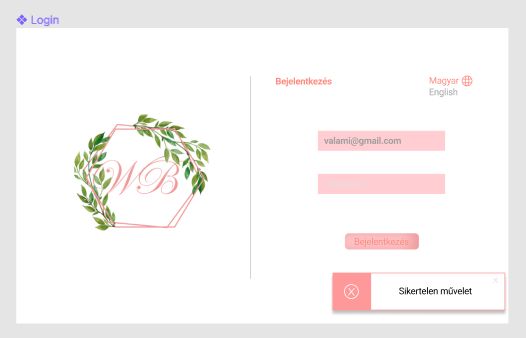
\includegraphics[width=0.45\textwidth]{images/login.png}}
	\hspace{5pt}
	\subcaptionbox{Termékek vázlatterve}{
		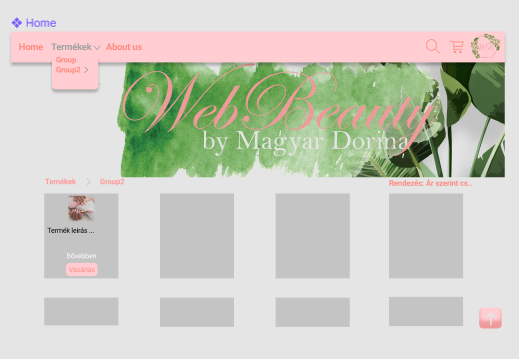
\includegraphics[width=0.45\textwidth]{images/oldal_terv.png}}
	\caption{Figma kiegészítő elemek tervezete}
	\label{fig.picture-12}
\end{figure}

\subsection{Logók és grafikai elemek}
Az alkalmazás grafikai elemeinek elkészítése során próbáltam figyelembe venni a program letisztult megjelenését és természetesen annak színvilágát. A webáruházban végül két különböző színű logó kerül felhasználásra. A \ref{fig.picture-13}-as ábra bal oldalán sötétebb kerettel és szöveggel rendelkező logó látható, amit a jobb oldali képpel megegyező színű háttereken használok. Ilyen háttérrel rendelkezik például az oldal menüsora. A jobb oldali logót fehér háttereken használom, mint például az adminisztrációs rész bejelentkezési felülete.
\begin{figure}[H]
	\centering
	\subcaptionbox{Sötétebb logó}{
		
\includegraphics[width=0.45\textwidth]{images/logo_monogram_dark.png}}
	\hspace{5pt}
	\subcaptionbox{Logó}{
		
\includegraphics[width=0.45\textwidth]{images/logo_monogram.png}}
	\caption{Grafikai elemek - logók}
	\label{fig.picture-13}
\end{figure}

A webshopon megjelenő további grafikai elemek, például a \ref{fig.picture-14}-es ábrán található képek célja, hogy változatosabb megjelenést kölcsönözzenek az alkalmazás számára.
\begin{figure}[H]
	\centering
	\subcaptionbox{Rólunk felület fejléce}{
		
\includegraphics[width=0.45\textwidth]{images/logo_name.png}}
	\hspace{5pt}
	\subcaptionbox{Főoldal felület fejléce}{
		
\includegraphics[width=0.45\textwidth]{images/logo_page_header.png}}
	\caption{Grafikai elemek}
	\label{fig.picture-14}
\end{figure}

\section{Forráskódok}
\label{section:sourcecode}

\subsection{Kliensoldali forráskódok}
\label{subsection:clientsource}
Ebben az alfejezetben található a \ref{section:client}-as fejezetben említett chatbot bemutatása forráskódok segítségével. Ez a funkció úgy került megvalósításra, hogy előre megírt és az adatbázisban eltárolt kérdéseket és válaszokat jelenítek meg animációk segítségével. Az alábbi forráskódrészletek ennek a megjelenítését írják le.

\bigskip
Először is lekérdezem és eltárolom ezt a chat listát a GET/chat~\ref{src:chat} forráskódban szereplő függvény segítségével.

\lstset{caption={GET/chat lista lekérés - TypeScript}, label=src:chat}
\begin{lstlisting}[language=JavaScript]
	async ngOnInit() {
		await this.chat.getChat();
		this.chatSub = this.chat.getUpdateListener()
		.subscribe(chat => {
			this.chatList = chat;
		});
	}
\end{lstlisting}

Ezután megjelenítem a listában szereplő kérdéseket HTML fájlban a \ref{src:chatHTML} forráskódban látottak szerint. Ezek a kérdések linkként szolgálnak, amik átirányítanak a kérdés animált profil oldalára, ami a \ref{src:chatProfile} forráskódban látható.
\lstset{caption={Chatbot megjelenítése - HTML}, label=src:chatHTML}
\begin{lstlisting}[language=html]
	<div class="chat-body">
	<div class="chat-link" *ngFor="let chat of chatList">
	<div (click)="loadChatProfile(chat.id)">{{chat.title}}</div>
	</div>
\end{lstlisting}

\lstset{caption={Chatbot kérdéshez tatoró szöveg megjelenítése - HTML}, label=src:chatProfile}
\begin{lstlisting}[language=html]
	<div class="animated display-message">
	<div class="chat__message chat__message_B" style="--delay: 2s">
	<div class="chat__content">
	{{selectedChat.title}}
	</div>
	</div>
	<div class="chat__message chat__message_A" style="--delay: 6s">
	<div class="chat__content">
	{{selectedChat.description}}
	</div>
	</div>
	...
\end{lstlisting}

A beszélgetés imitálásához SCSS-ben írt stílusfájlt használtam a \ref{src:scss} forráskódban leírtak alapján.

\lstset{caption={Chatbot beszélgetés animáció - SCSS}, label=src:scss}
\begin{lstlisting}
	.chat__message {
		...
		transform-origin: 0 100%;
		padding-top: 0;
		transform: scale(0);
		...
		animation: message 0.15s ease-out 0s forwards;
		animation-delay: var(--delay);
		--bgcolor: var(--info-color);
		--radius: 8px 8px 8px 0;
	}
	
	.chat__message_B{
		color: var(--light-color);
		flex-direction: row-reverse;
		text-align: right;
		align-self: flex-end;
		transform-origin: 100% 100%;
		--bgcolor: var(--main-color);
		--radius: 8px 8px 0 8px;
	}
	
	.chat__message::before {
		content: "";
		flex: 0 0 40px;
		aspect-ratio: 1/1;
		background: var(--bgcolor);
		border-radius: 50%;
	}
\end{lstlisting}

\subsection{Szerveroldali forráskódok}
\label{subsection:serversource}
Az alább található forráskódok a \ref{subsection:restapi}-es fejezetben említett JavaScript programozási nyelv segítségével írt példa lekérések láthatóak. A programban használt végpontok, amik bemutatásra kerülnek ebben a fejezetben a következő kérések: GET, DELETE és PUT műveletek.

GET/news~\ref{src:get}-es forráskódban látható a GET végpont lekérése, aminek segítségével lekérésre kerül az adatbázisból a hírek listája. Az adatbázis válaszüzenetben visszaküld egy JSON fájlt. Ez a JSON fájl a \ref{src:getJSON}-es forráskód leírásában látható.

\lstset{caption={GET/news végpont}, label=src:get}
\begin{lstlisting}[language=JavaScript]
	exports.getChat = (req, res, next) => {
		Chat.find().then(result => {
			res.status(200).json({
				message: "Chat fetched successfully",
				chat: result,
			});
		});
	}
\end{lstlisting}

\lstset{caption={GET/news JSON}, label=src:getJSON}
\begin{lstlisting}[language={JSON}]
	{
		"message": "News fetched successfully!",
		"news": [
		{
			"_id": "61b61edfb415f9f7cc07e7a8",
			"title": "Oldal letrehozasa",
			"description": "Az oldal letrehozasa Magyar Dorina Szakdolgozata elkeszitese celjabol tortent. Jelenleg ez az oldal nem uzemel! Nem kerulnek ertekesitesre azok a termekek, amik az aruhazban talalhatoak! Ha tovabbi kerdese lenne a Rolunk feliratu menun keresztul kapcsolatba lephet velem es minden kerdesre email formajaban valaszolok. Megerteseteket elore is koszonom!",
			"imagePath": "http://localhost:3000/images/news/oldal-letrehozasa-1639325407045.png",
			"startDate": "2021-08-31T22:00:00.000Z",
			"endDate": "2021-12-14T23:00:00.000Z",
			"__v": 0
		}, ...
		]
	}
\end{lstlisting}

PUT/news~\ref{src:put}-es forráskódban szereplő módosítás művelet végpontja látható. Ennek a végpont segítségével képesek vagyunk módosítani az adatbázisban szereplő lista elemeit. Az adatbázis válaszüzenetben visszaküldi a művelet státuszát. Ha sikeresként tér vissza akkor a \ref{src:putJSON}-es forráskódban szereplő JSON objektumot kapjuk meg.

\lstset{caption={PUT/news végpont}, label=src:put}
\begin{lstlisting}[language=JavaScript]
	exports.putNews = (req, res, next) => {
		let imagePath = req.body.imagePath;
		if(req.file) {
			const url = req.protocol + "://" + req.get("host");
			imagePath = url + "/images/news/" + req.file.filename
		}
		const news = new News({
			_id: req.body.id,
			title: req.body.title,
			description: req.body.description,
			imagePath: imagePath,
			startDate: req.body.startDate,
			endDate: req.body.endDate,
		});
		News.updateOne({_id: req.params.id}, news).then(result => {
			res.status(200).json(
			{message: "Update succsessful!"}
			);
		});
	}
\end{lstlisting}

\lstset{caption={PUT/news JSON}, label=src:putJSON}
\begin{lstlisting}[language={JSON}]
	{
		"message": "Update succsessful!",
		"news": [
		{
			"_id": "61b61edfb415f9f7cc07e7a8",
			"title": "Oldal letrehozasa valtozas",
			"description": "Az oldal letrehozasa Magyar Dorina Szakdolgozata elkeszitese celjabol tortent. Jelenleg ez az oldal nem uzemel! Nem kerulnek ertekesitesre azok a termekek, amik az aruhazban talalhatoak! Ha tovabbi kerdese lenne a Rolunk feliratu menun keresztul kapcsolatba lephet velem es minden kerdesre email formajaban valaszolok. Megerteseteket elore is koszonom!",
			"imagePath": "http://localhost:3000/images/news/oldal-letrehozasa-1639325407045.png",
			"startDate": "2021-08-31T22:00:00.000Z",
			"endDate": "2021-12-14T23:00:00.000Z",
			"__v": 0
		}]
	}
\end{lstlisting}

DELETE/news~\ref{src:delete}-as forráskódban a DELETE kérés végpontja szerepel. Ezzel a művelettel lehetőségünk van kitörölni az adatbázisból az átadott paraméterrel rendelkező adatokat. Válaszüzenetként csak a kérés státuszát kapjuk vissza.

\lstset{caption={DELETE/news végpont}, label=src:delete}
\begin{lstlisting}[language=JavaScript]
	exports.deleteNews = (req, res, next) => {
		News.deleteOne({_id: req.params.id}).then( result => {
			res.status(200).json({
				message: "News deleted!"
			});
		});
	}
\end{lstlisting}

\section{Tesztesetek}

\subsection{Kliensoldal tesztelése}
A kliensoldal tesztelésére általam végrehajtott felülettesztelést végeztem. A felhasználói felülettesztelést gyakran használják webes alkalmazások tesztelésére. Ennek a módszernek a lényege, hogy a felületet állandó stressznek tesszük ki.

\begin{enumerate}
	\item\label{step:first} A bejelentkezési felület tesztelése: a \ref{fig.picture-15}-ös ábra bal oldalán látható képen helyesen megadott emailcím és jelszó párossal próbálok belépni, ami sikeres üzenettel tér vissza. A sikeres teszt eredményeként átnavigál az adminisztrációs felület termékek listája oldalra. Az ábra jobb oldalán helytelen adatok megadásával sikertelen művelet üzenettel tér vissza az oldal. A sikertelen teszt eredményeként a bejelentkezési kérelem elutasításra kerül és ezen a felületen marad.
	\begin{figure}[H]
		\centering
		\subcaptionbox{Sikeres bejelentkezési művelet}{
			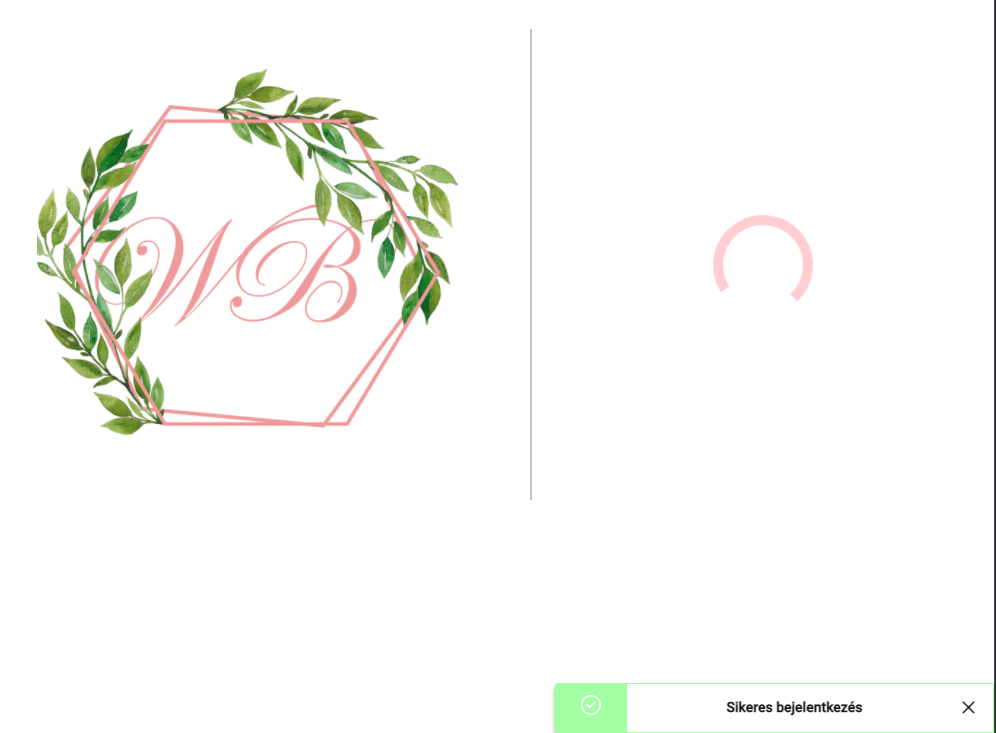
\includegraphics[width=0.45\textwidth]{images/sikeres_bejelentkezes.png}}
		\hspace{5pt}
		\subcaptionbox{Sikertelen bejelentkezési művelet}{
			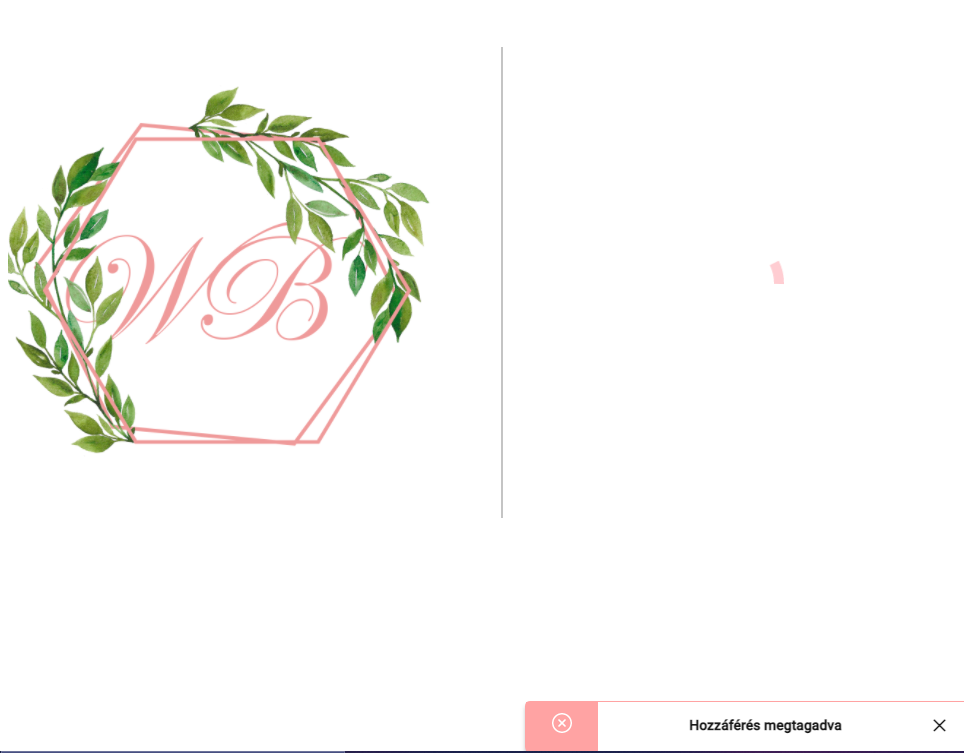
\includegraphics[width=0.45\textwidth]{images/sikertelen_bejelentkezes.PNG}}
		\caption{Bejelentkezési felület tesztelése}
		\label{fig.picture-15}
	\end{figure}
	\item Reszponzivitás: az oldal telefonon, táblagépen és asztaligépen is megfelelően tölti be az oldalt. A megjelenése eszközspecifikusan reszponzív. A \ref{fig.picture-16}-os ábra bal oldala a telefonos nézetet jeleníti meg, míg az ábra jobb oldala a táblagépről látott képet mutatja be. Mindkettő kép esetében láthatjuk, hogy a menüsor elrejtésre kerül. Ezzel biztosítva azt, hogy nem csúszik össze az ikonokkal. Az ábrán továbbá megfigyelhető, hogy a hírek és a termékek listája módosítva jelenik meg. Mindkét eszköz felületén a termékek kártyái láthatóan újra rendeződnek. Továbbá mobilnézetben a főoldalon megjelenő hírek és az azokhoz tartozó képek elrejtésre kerülnek.
	\begin{figure}[H]
		\centering
		\subcaptionbox{Alkalmazás telefonos nézete}{
			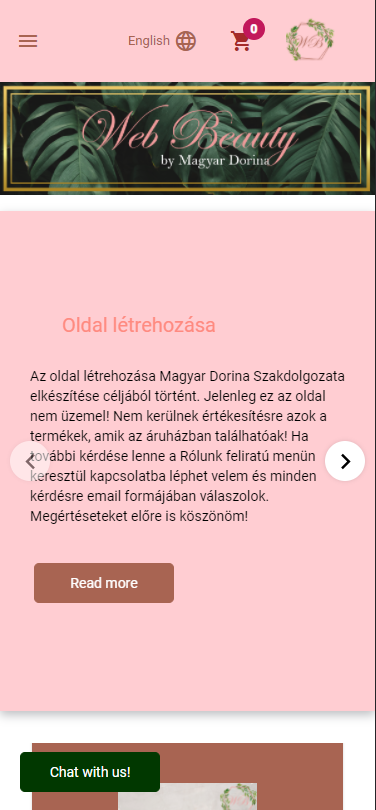
\includegraphics[width=0.45\textwidth]{images/responsive_mobile.PNG}}
		\hspace{5pt}
		\subcaptionbox{Alkalmazás táblagépes nézete}{
			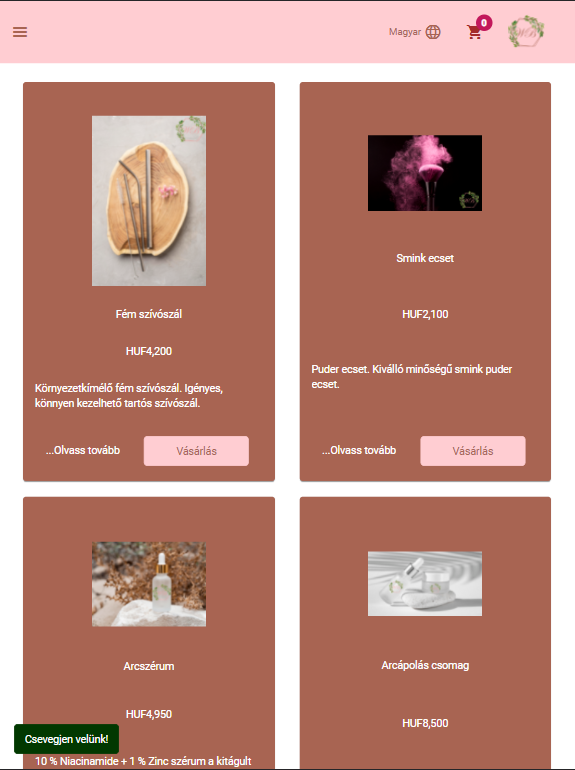
\includegraphics[width=0.45\textwidth]{images/responsive_tablet.PNG}}
		\caption{Reszponzív felület tesztelése}
		\label{fig.picture-16}
	\end{figure}
\end{enumerate}


\subsection{Szerveroldal tesztelése}
Az alábbi fejezetben látható a szerveroldalon megírt REST API kérések tesztelése látható táblázat formájában. A végpontok tesztelését Postman\cite{postman} program segítségével készítettem. A \ref{tab:example-4} táblázat első oszlopában látható a kérésekre vonatkozó hitelesítési kötelezettségük. A második oszlopban a kérések URL címe olvasható, ezekkel a címekkel érhetőek el a back-enden megírt függvények. A harmadik és negyedik oszlopban ezeknek a kéréseknek a végrehajtás státuszáról látható válaszüzenetek. Ilyen információ például az, hogy sikeres volt-e a művelet, és milyen üzenet társul hozzá.

\begin{table}[H]
	\begin{tabular}{ | c | l | c | l | }
		\hline
		\multicolumn{4}{|c|}{\textbf{Szerveroldali végpontok tesztelése}}
		\\ \hline
		\hline
		\multicolumn{4}{|c|}{\textbf{GET}} \\
		\hline
		\multicolumn{1}{| c |}{\textbf{ Token }} & \multicolumn{1}{ c |}{\textbf{Request URL}} & \multicolumn{1}{ c | }{\textbf{Status}} & \multicolumn{1}{ c | }{\textbf{Message}} \\
		\hline		
		nem & api/products & 200 OK & Products fetched successfully  \\
		\hline
		nem & api/productsGroups &200 OK & Group fetched successfully \\
		\hline
		nem & api/news & 200 OK & News fetched successfully \\
		\hline
		nem & api/chat & 200 OK & Chat fetched successfully  \\
		\hline 
		nem & api/messages & 401 Unauthorized & Auth failed  \\
		\hline 
		igen & api/messages & 200 OK & Message fetches successfully  \\
		\hline
		igen & api/orders & 200 OK & Order fetches successfully \\
		\hline
		\multicolumn{4}{|c|}{\textbf{POST}} \\
		\hline
		\multicolumn{1}{| c |}{\textbf{ Token }} & \multicolumn{1}{| c |}{\textbf{Request URL}} & \multicolumn{1}{ c | }{\textbf{Status}} & \multicolumn{1}{ c | }{\textbf{Message}} \\
		\hline
		igen & api/products & 500 Server Error & Unexpected field \\
		\hline
		igen & api/products & 200 OK & Products added successfully \\
		\hline
		igen & api/news & 200 OK & News added successfully \\
		\hline
		nem & api/messages & 200 OK & Message added successfully \\
		\hline
		nem & api/orders & 200 OK & Products added successfully \\
		\hline
		\multicolumn{4}{|c|}{\textbf{PUT}} \\
		\hline
		\multicolumn{1}{| c |}{\textbf{ Token }} & \multicolumn{1}{| c |}{\textbf{Request URL}} & \multicolumn{1}{ c | }{\textbf{Status}} & \multicolumn{1}{ c | }{\textbf{Message}} \\
		\hline
		igen & api/products & 500 Server Error & Unexpected field \\
		\hline
		igen & api/products & 200 OK & Update successful \\
		\hline
		igen & api/news & 200 OK & Update successful \\
		\hline
		\multicolumn{4}{|c|}{\textbf{DELETE}} \\
		\hline
		\multicolumn{1}{| c |}{\textbf{ Token }} & \multicolumn{1}{| c |}{\textbf{Request URL}} & \multicolumn{1}{ c | }{\textbf{Status}} & \multicolumn{1}{ c | }{\textbf{Message}} \\
		\hline
		igen & api/products/6186.. & 200 OK & Products deleted \\
		\hline
		igen & api/news/61ae.. & 200 OK & News deleted \\
		\hline
		igen & api/messages/61a4.. & 200 OK & Message deleted \\
		\hline
		igen & api/orders/6197.. & 200 OK & Order deleted \\
		\hline
		
	\end{tabular}
	\caption[Szerveroldali végpontok tesztelése]{Back-end REST API kérés végpontok tesztelése.}
	\label{tab:example-4}
\end{table}


\section{Továbbfejlesztési lehetőségek}
Az alkalmazás továbbfejlesztés céljaként szeretném a webáruház felületén is megjeleníteni az autentikációt. Ezzel lehetővé téve, hogy a vásárlók létrehozzák a saját fiókjukat, aminek a segítségével láthatják a vásárlási előzményeiket. Bejelentkezés után a vásárlók, egy ajánlott terméklistát láthatnának az előzményeik alapján leszűrve, továbbá mások által együtt vásárolt termékek intelligens összekötése és ajánlása további vásárlók számára. A program mostani verziójába azért nem került be ez a funkció a webshop felületére, mert jelenleg nem tudnám különválasztani az adminisztrációs és a webáruház felület bejelentkezését. A későbbiekben erre a problémára megoldásként szolgálhat a szerepkörök bevezetése.
\cleardoublepage

\chapter{Összegzés} % Conclusion
\label{ch:sum}

A program sikeresen bemutat egy működő webáruházat, amit kisvállalkozók saját termékeik értékesítésére alkalmas. Az alkalmazást első sorban egy vállalkozó általi megkeresés céljából készítettem el. De a fejlesztés során számos új technológiákat és új módszereket sikerült megismernem, amikel az egyetemi tanulmányaim során nem találkoztam. Az alkalmazás megvalósítására használt MEAN szoftverköteg nem egyedi, hiszen rengeteg projektnek az alapjaként szolgál, még is a kliensoldalon használt kiegészítő csomagjainak segítségével egy hangulatos elsősorban kozmetikai eszközök értékesítését szolgáló webáruházat sikerült lefejlesztenem. Viszont a későbbiekben az alkalmazás képes kiszolgálni más megjelenést és tartalmi igényeket kérő projekteket, mivel ezek az adatok dinamikusan vannak kezelve. Az adminisztrációs rész megkönnyíti a vállalkozó számára a felület karbantartását, hiszen felhasználóbarát módosítási lehetőségek kerültek implementálásra. A használt technológiák megfelelő kompatibilitással rendelkeznek egymással szemben. Ennek köszönhetően nem ütköztem nagyobb akadályokba a fejlesztés során.

\bigskip
Külön megszeretném köszönni Nemesné Balla Júlia Évának, hogy lehetőséget kaptam az alkalmazás elkészítésére. Továbbá szeretném megköszönni Fekete Anett PhD hallgatónak, hogy elvállalta a szakdolgozatom témavezetését és végig támogatta a program elkészítését.
\cleardoublepage

% Függelékek (opcionális) - hosszabb részletező táblázatok, sok és/vagy nagy kép esetén hasznos
% Appendices (optional) - useful for detailed information in long tables, many and/or large figures, etc.
%\appendix
%\input{appendices/sim.tex}
%\cleardoublepage

% Irodalomjegyzék (kötelező)
% Bibliography (mandatory)
\phantomsection
\addcontentsline{toc}{chapter}{\biblabel}
\printbibliography[title=\biblabel]
\cleardoublepage

% Ábrajegyzék (opcionális) - 3-5 ábra fölött érdemes
% List of figures (optional) - useful over 3-5 figures
\phantomsection
\addcontentsline{toc}{chapter}{\lstfigurelabel}
\listoffigures
\cleardoublepage

% Táblázatjegyzék (opcionális) - 3-5 táblázat fölött érdemes
% List of tables (optional) - useful over 3-5 tables
\phantomsection
\addcontentsline{toc}{chapter}{\lsttablelabel}
\listoftables
\cleardoublepage

% Algorithmusjegyzék
% List of algorithms
%\phantomsection
%\addcontentsline{toc}{chapter}{\lstalgorithmlabel}
%\listofalgorithms
%\cleardoublepage

% Forráskódjegyzék (opcionális) - 3-5 kódpélda fölött érdemes
% List of codes (optional) - useful over 3-5 code samples
\phantomsection
\addcontentsline{toc}{chapter}{\lstcodelabel}
\lstlistoflistings
\cleardoublepage

% Jelölésjegyzék (opcionális)
% List of symbols (optional)
%\printnomenclature

\end{document}
